\documentclass[a4paper]{article}
\usepackage[utf8]{inputenc}
\usepackage[dvipsnames]{xcolor}
\usepackage[hidelinks]{hyperref}
\usepackage{graphicx, amssymb, amsfonts, color, todonotes, diagbox, colortbl, pdfpages, listings, amsmath, caption, subcaption, xspace, xcolor, pifont, fullpage, algorithm, algpseudocode}
\algnewcommand\algorithmicforeach{\textbf{for each}}
\algdef{S}[FOR]{ForEach}[1]{\algorithmicforeach\ #1\ \algorithmicdo}
\setlength{\parskip}{0.2 cm}
\newtheorem{definition}{Definition}
\newtheorem{theorem}{Theorem}

% Commands
\newcommand{\Node}[1]{\ensuremath{\mathrm{Node}_{#1}}\xspace}
\newcommand{\flow}[1]{\ensuremath{\mathit{flow}_{#1}}\xspace}
\newcommand{\inputs}{\ensuremath{\mathcal{F}}\xspace}
\newcommand{\memory}{\ensuremath{\mathcal{M}}\xspace}
\newcommand{\memorymap}{\ensuremath{\mathcal{M}_{map}}\xspace}
\newcommand{\duration}{\mathit{Duration}\xspace}
\newcommand{\bandwidth}{\mathit{BW}\xspace}
\newcommand{\core}{\mathit{Cores}\xspace}
\newcommand{\submissiontime}{\mathit{Subtime}\xspace}
\newcommand{\walltime}{\mathit{Walltime}\xspace}
\newcommand{\completiontime}{\mathit{Completiontime}\xspace}
\newcommand{\start}{\mathit{Starttime}\xspace}
\newcommand{\fileset}{\ensuremath{\mathbb{F}}\xspace}
\newcommand{\jobset}{\ensuremath{\mathbb{J}}\xspace}
\newcommand{\evict}{\ensuremath{\mathcal{V}}\xspace}
\newcommand{\nbloads}{\ensuremath{\mathit{\mathit{Loads}}}\xspace}
\newcommand{\live}{\ensuremath{L}\xspace}
\renewcommand{\algorithmicrequire}{\textbf{Input:}}
\renewcommand{\algorithmicensure}{\textbf{Output:}}

\title{Data Aware Batch Scheduling}
\author{Maxime GONTHIER - Carl NETTELBLAD - Elisabeth LARSSON \\ Samuel THIBAULT - Loris MARCHAL}
\usepackage[backend=bibtex]{biblatex}
\bibliography{ref}

\begin{document}

\maketitle
\tableofcontents
\listoffigures
\newpage

\todo[inline]{Maxime: You can add highlighted comments this way: "\textbackslash todo[inline]\{Text\}".}
\todo{Maxime: Or with: "\textbackslash todo\\\{Text\}".}

\section{Motivation}

When using a HPC cluster, users may submits tens to hundreds jobs using the same multi-GB input file.
Users tend to submit each such run as a separate batch job.
The job will read inputs directly from a shared file system, which can be disastrous if the number of I/O are important.
We can thus ask ourselves, \textbf{how can we minimize the amount of transfers between the shared file system and the nodes ?}

Users can manually group together input files into a single job to reduce the effects from I/O reads.
Ideally, we would like to let the user submit jobs the way they want and schedule efficiently jobs on nodes.
The workers have a way to store files (with a limit on the memory size), as well as a cache page which contains the files/data recently used.
Thus, a way to minimize data transfers is to create a scheduler that \textbf{take into consideration data locality and schedule on the same node jobs sharing inputs}.

Our scheduler would be used to \textbf{distribute the load between the workers but also to have a vision of what the memory of each worker contains in order to re-use as much as possible a file already loaded on a worker's local memory}.

Clusters already use the efficient SLURM scheduler in order to distribute jobs.
\textbf{Thus our goal is to add a scheduler before the SLURM scheduler that would allocate to each job a node.}

\section{Related Work}

\subsection{About SLURM}
SLURM~\cite{SLURM} is a cluster resource management system, flexible, fault-tolerant and highly scalable.
Schedulers are part of the standard configuration. The Backfill algorithm is very widely used~\cite{New_Backfill}.
Backfill is based on the First Come - First Served principle. While the scheduler is running, jobs in the queue are sorted by priority and queueing time~\cite{New_Backfill}.
If there are not enough nodes to start a job, Backfill takes the next job from the queue and sets it for execution if there are enough nodes for this job and 
it does not delay other jobs.
This algorithm allows to increase the density of supercomputer ressources' use by 20\% as well as reducing the average waiting time
for execution~\cite{Maui_Scheduler}.
Thus our starting point can be the Backfill algorithm.
To be precise, we will be using EASY-Backfilling, a scheduler known to be efficient and able to prevent starvation~\cite{easybf}.
\textbf{We will add a data-aware strategy that maximize data reuse while maintaining EASY-Backfill's basic principle.}

\subsection{Improving SLURM and other batch systems}
To deal with communication-intensive jobs on SLURM, a solution is to minimize network contention by allocating nodes on the least
contended switches~\cite{minimize_network_contention}. In our case we have
jobs with one large file transfers that must be done before the computation start, which is different.
Furthermore, we are scheduling further down the topology (i.e nodes and not switches).

In "Explicit Control in a Batch-Aware Distributed File System"~\cite{Explicit_Control_in_a_Batch-Aware_Distributed_File_System},
we are presented with "Batch-Aware Distributed File System", a system designed to orchestrate large, 
I/O-intensive batch workloads on remote computing clusters.
It adds "storage servers" that export access to the disk. And a scheduler that
manage jobs. 
Like us, they use detailed knowledge of workload characteristics.
However, the main idea is not data reuse but to
facilitates the execution of I/O intensive batch
jobs by selecting appropriate storage policies
in regards to I/O scoping (creating a custom environment for each job
for data that will be used a lot by the job, thus not accessing the main disk too
much) and space allocation.


\subsection{About memory-aware scheduling}
Memory-aware scheduling on clusters have been studied in the past.
 
"Algorithmic Modifications to the
Jacobi-Davidson Parallel Eigensolver to Dynamically Balance External CPU and Memory Load"~\cite{loadbalance_and_trashing} tackle both load balancing and memory constraint. For the load balancing, they 
estimate the time needed by the fastest processor to perform the required $m$ jobs. Thus they can equilibrate the load
with this information. In our study we could use a similar strategy by estimating the 
processing time of a job, the length of a file transfer, and the amount of file transfers needed.
To deal with memory constraint the strategy applied in the paper is to check if 
nodes are thrashing data. If yes, it will recede execution of jobs on this node.
The main differences are that they are using dynamic jobs. Also, we would like to 
manage eviction and optimize data reuse during the scheduling phase, instead of
receding execution on nodes.

Some researchers~\cite{Nikolopoulos2003AdaptiveSU}
are focusing on a better utilization of idling memory together with 
thrashing limitation. Our focus will be to control data loads and eviction so the
processing order will naturally limits thrashing.

\subsection{HDFS, a popular distributed file system}
HDFS~\cite{hdfs} or Hadoop Distributed File System is a distributed file system that incorporate memory-aware scheduling.
HDFS is suitable for applications that have large data sets. 
"Moving Computation is Cheaper than Moving Data" is an important idea for HDFS.
It will migrate a computation closer to where the data is located rather than moving the data to where
the application is running.
Here are our main differences with HDFS. Firstly, HDFS is made for commodity hardware, prone
to more errors and breakdown, so to minimize the risk of failure, data are redundant on the nodes.
In our use case, the scheduler will run on professional clusters and the main point is to load as 
little data as possible. Secondly, HDFS is mainly a storage system, with metadata as transactions historic or
block location. Those concept are not relevant in our use case. Thirdly, the scheduling 
can have issues. A paper describe in detail some problems from MapReduce~\cite{issue_with_hdfs}, the
programming language used in HFDS: the static configuration of the memory allocation, the one-task assigned buffers, the
lake of concurrent task running strategy and the I/O negative impact in memory during the shuffling phase.
To resolve these issues, Mammoth~\cite{Mammoth} was created. It optimize memory usage on a node depending on the hardware configuration.
Our approach is different because we are not dealing with MapReduce or memory allocation.
Our approach is upstream. We can only allocate jobs to nodes. Moreover, we would like to maintain
equity among users  while optimizing I/O.
In addition, HDFS is particularly efficient when the input data used are identical over time.
In our case, one user will submit a lot of different jobs using the same data, but between users,
the inputs are not the same. So HDFS would be less efficient.


\section{Problem Modeling}

\subsection{Framework}
We consider the problem of scheduling independent jobs $J$ on $K$ nodes,
denoted by $\Node{1},\ldots, \Node{K}$.
Each node is equipped with 20 cores noted: $\Node{1}(C_1, C_2, ..., C_{20})$.
Each node has a limited memory $\memory(\Node{i})$ of size 1TB, 256GB or 128GB.
We denote by $\fileset$ the set of input files and $\jobset$ the set of jobs.
We denote by $\inputs(J_i)$ the input file required by job $J_i$. $\inputs(J_i)$ can be empty.
Each file has a size in GB noted $\memory(F_i)$. 
Each job request a certain number of cores $\core(J_i)$. 


Only jobs using 5 cores or more have input files.
If multiple jobs are submitted by the same user on a short period of time (less than 30 seconds between each job),
then those jobs will share the same input file.
The size of an input file is proportional to the number of cores required.
Each job has a certain probability of requiring cores of sizes 128GB, 256GB or 1024GB.
Thus, the size of a file can be:
\begin{itemize}
	\item If $\core(J_i) < 5$:
	\begin{itemize}
		\item $0GB \times \core(J_i)$, requiring either the 128GB, 256GB or 1024GB node.
	\end{itemize}
	\item If $\core(J_i) \ge 5$:
	\begin{itemize}
		\item $6.4GB \times \core(J_i)$, requiring either the 128GB, 256GB or 1024GB node.
		\item $12.8GB \times \core(J_i)$, requiring either the 256GB or 1024GB node.
		\item $51.2GB \times \core(J_i)$, requiring exclusively 1024GB node.
	\end{itemize}
\end{itemize}
With this model, a job cannot have a file larger than 1024GB.
Also with this model there cannot be any situation in which the memory is fully used
but the cores are not. Because these two values are related to each other. 
However we can have situation where the memory is not fully used but the cores are,
for example if a 20 core job using 128GB memory is schedule on the 1024GB node.

Each job has a submission time $\submissiontime(J_i)$ and a walltime $\walltime(J_i)$.
A job can request between 1 and 20 cores.
Each job using input files is using a shared file.

Initially, all input files are stored in the main shared file system.
During the processing of a job $J_i$ on $\Node{k}$, all its inputs
$\inputs(J_i)$ must be in the memory of $\Node{k}$. 
We do not consider the data output of jobs.
Each of the $m$ jobs must be processed on some of the $K$ nodes. 
We consider that all jobs are single nodes.

The file sharing system initially contains all of $\fileset$.
Each node is connected to the file sharing system with a limited bandwidth.
Each node has the same bandwidth noted $\bandwidth$ which is equal to 0.1 GB/s.
The bounded bandwidth as well as the sizes of the files are the reasons why
we aim at restricting the amount of data movement.

The memory of a node is used only by physical writing of files and denoted by $\memory(\Node{i})$.
A file can be shared by two jobs $J_i$ and $J_j$ only in the following situations:
\begin{enumerate}
	\item $J_i$ and $J_j$ are computed in parallel on the same node.
	\item $J_i$ and $J_j$ are computed on the same node consecutively.
	\item $J_i$ and $J_j$ are computed on the same node and between the end of $J_i$ and the beggining of $J_j$, no other job is being computed.
\end{enumerate}
Otherwise we consider that memory operations will cause the files to be evicted.
When a node is idling however, we consider that we can enforce a policy that will
pin unoccupied address space containing the last input file that was used.
This input file will be "free" to use for the next job schedule on the node. It correspond to point number 3.

We now define more formally the allocation of the jobs to the node and
their schedule.
We denote by $\sigma(k,i)$ the $i^\text{th}$ job
processed on $\Node{k}$ and by $\evict(k,i)$ the set of file to
be evicted from the memory of $\Node{k}$ before the processing
of this $i^\text{th}$ job ($\evict(k,i)$ can be empty if there is enough space to fit the new files).

On $\Node{k}$, the schedule is made of a
succession of $\mathit{nb}_k$ (the number of jobs allocated) steps, each step being composed of the
following stages (in this order):
\begin{enumerate}
%~ \item Eviction of files if the memory is saturated (we can use flags to force a file to stay in memory. In the same way, we can add a "won't use" flag on a file in order to evict it);
\item The input files in $\inputs(J_{\sigma(k,i)})$ that are not yet in memory are loaded in the memory of $\Node{k}$;
\item Job $J_{\sigma(k,i)}$ is processed on $\Node{k}$ during at most $\walltime(J_i)$.
\end{enumerate}
It is important to note that the file transfers are done before the computation and can not be overlapped.

%~ We define the \emph{live data} $\live(k,i)$
%~ as the files in memory of $\Node{k}$ during the computation of $J_{\sigma(k,i)}$, which
%~ can be defined recursively:
%~ $$
%~ \live(k,i)=
%~ \begin{cases}
  %~ \inputs(J_{\sigma(k,1)}) & \text{if~}i=1\\
%~ \Big(\live(k,i-1) \backslash \evict(k,i)\Big) \cup \inputs(J_{\sigma(k,i)})
%~ & \text{otherwise}
%~ \end{cases}
%~ $$

We are in a Non-Preemptive case, so we cannot stop a job and resume it later.

\subsection{Formalization of the objective}
\textbf{Objective: Minimize the maximum \flow{}}
		We define the \flow{J_i} of a job as:
		$$
			\flow{J_i} = \completiontime(J_i) - \submissiontime(J_i)
		$$
		Our goal is:
		$$
			\textbf{Obj.}: \quad \mathit{minimize}~\mathit{max}(\flow{J_1}, \flow{J_2}, ..., \flow{J_m})
		$$
A secondary objective is to minimize the amount of file loaded in MB.
Indeed, loading files has a huge impact on the total makespan and thus on the maximum \flow{}.

\section{Other measurements}

Each job has a start time $\start(J_i)$, the actual time at which the job was executed.
We also want to measure the average queue time of a job in order
to evaluate our scheduler in terms of fairness. We can do:
$$
	Average\_queue\_time = \frac{\sum^{m}_{i = 0} \start(J_i) - \submissiontime(J_i)}{m}
$$

%~ We also want to measure the core-hours used. We need to take into consideration the amount of files loaded before the computation.
%~ With $\core(J_i)$ the number of processor units used by job $i$ and $\duration(J_i)$ the duration of job $i$ in hours, we have:
%~ $$
	%~ \#Corehours = \sum^{m}_{i = 0} \core(J_i) \times (\duration(J_i) + \frac{\memory(\inputs\left(J_{\sigma(k,i)}\right) \backslash \live(k,i-1)))}{\bandwidth}
%~ $$

\section{The use of simulation}

The use of simulation is motivated both by the fidelity of simulated results as well as energy savings. 
We will be using Batsim, a precise and realistic~\cite{Batsim} resource and job management system (RJMS) simulator.
Batsim JSON-formatted workloads are extensible and allow easy workload generation. 
Moreover, Batsim provides clear information about scheduling metrics and job placement.
We will add a scheduler using Batsched~\footnote{\url{https://gitlab.inria.fr/batsim/batsched}}.

\paragraph{Data mining for an accurate simulation}
We are matching Uppsala's University cluster Rackham:
\begin{itemize}
	\item	Bandwidth of each node: Let's stick with 100 MB/s as the BW for writing
	\item	Size of input files: 800 to 0GB
	\item	Duration of jobs: from real data
	\item	Total number of jobs: from real data
	\item	Number of available nodes: 486 max. We can test with different number ranging from 20 to 486
	\item	Size of node's memory: 4 of 1TB, 32 of 256GB and the rest has 128GB : A file larger won't be accepted. You need to use the 1TB node if your file is too large.
\end{itemize}

\paragraph{How to simulate data transfers ?}
We can add dynamic job of duration the time it would take to transfer the file on the node in order
to simulate file loads.

\section{Algorithm}

When we need to choose a node for job $J_i$ we know the following informations:
\begin{itemize}
	\item $\submissiontime(J_i)$
	\item $\walltime(J_i)$
	\item $\inputs(J_i)$
	\item Size of files for the job: $\memory(\inputs(J_i))$
	\item For each $i$, $\inputs(\Node{i})$
	\item Size of files already on memory of the node: For each $i$, $\memory(\inputs(\Node{i}))$
	\item Bandwidth: $\bandwidth$
\end{itemize}

\subsection{Maximum use single file}
\paragraph{Intuition}
Find the file shared the most among available jobs.
Schedule all jobs using this file on a node using this file with most available cores.
\begin{algorithm}[H]
\caption{Maximum use single file}
\hspace*{\algorithmicindent} \textbf{Input: Set of available jobs $\jobset$ at time $t$} \\
\hspace*{\algorithmicindent} \textbf{Output: Schedule for each job}
\begin{algorithmic}[1]
\While{$\jobset != \emptyset$}
	\State Find file $F_j$ used by the most jobs in $\jobset$
	\State $\Node{selected} \gets$ node with most available cores such as $F_j \in \inputs(\Node{i})$ and $\memory(F_j) <= \memory(\Node{i})$
	\If{$\Node{selected} = \emptyset$}
		\State $\Node{selected} \gets$ node with most available cores such as $\memory(F_j) <= \memory(\Node{i})$
	\EndIf
	\ForEach {$J_i \in \jobset$ such as $F_j \in \inputs(J_i)$}
		\State Schedule $J_i$ on $\Node{selected}$ on the earliest available core(s)
		\State Remove $J_i$ from $\jobset$
	\EndFor
\EndWhile
\end{algorithmic}
\end{algorithm}

\subsection{Distribute files}
\paragraph{Intuition}
The goal is to distribute files on a certain number of nodes in order to equilibrate the load
and have multiple choices when choosing a node.

Let's say we have 50 nodes.

Compute the number of copy of each file among each nodes.

If a file is already loaded on 10 or more nodes, jobs using this 
file can only be scheduled on the first available cores among those nodes.

If a file is loaded on less than 10 nodes, jobs using this file are scheduled on nodes 
that are not using this file and that have the most memory available left,
until there are 10 nodes using this file. After that, jobs are schedule on nodes using this file.

\subsection{FCFS with a score}
\paragraph{Intuition}
Choose the job j submitted the earliest.

For each node, A = compute the earliest available time to host job j.

For each node, B = compute the time it will take to load all the files from j not yet in memory.

For each node, C = compute the amount of data that will need to be evicted to load all the files from j not yet in memory. These files will need to be re loaded for other jobs.

Each node get a score combining these three values: Score = A + B + (C/BW)

Schedule j on the node with the best score.

\section{Stats on workloads for Rackham}

% Cores
\begin{figure}[H] 
  \begin{minipage}[b]{0.5\linewidth}
    \centering
    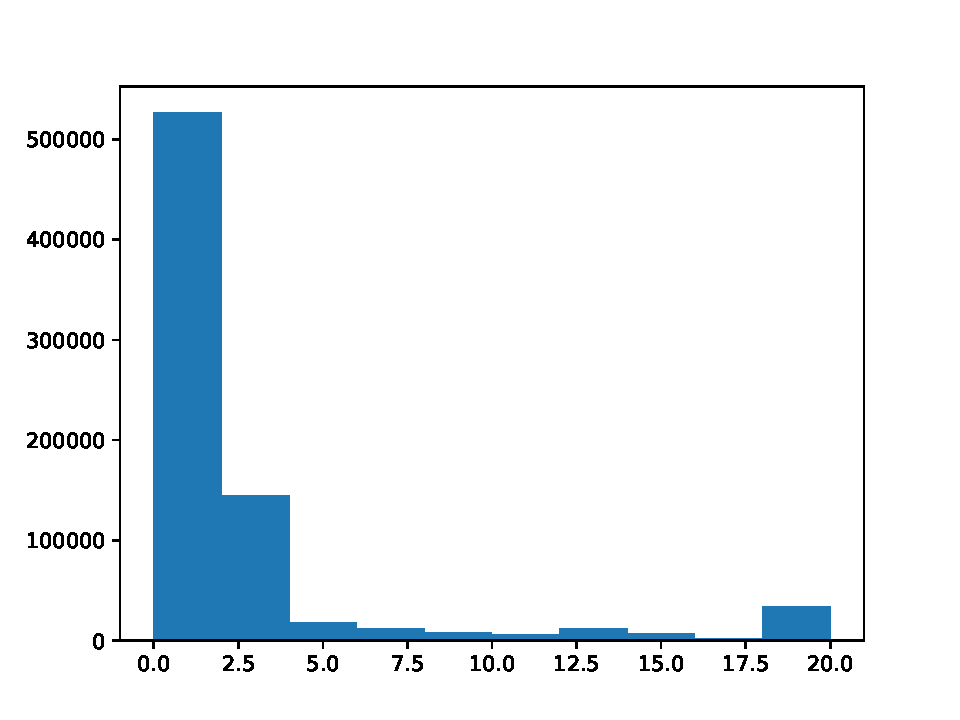
\includegraphics[width=1.11\linewidth]{MBSS/plot/Distribution/2022_01_cores.pdf} 
    \caption{Cores - January 2022} 
    \vspace{4ex}
  \end{minipage}%%
  \begin{minipage}[b]{0.5\linewidth}
    \centering
    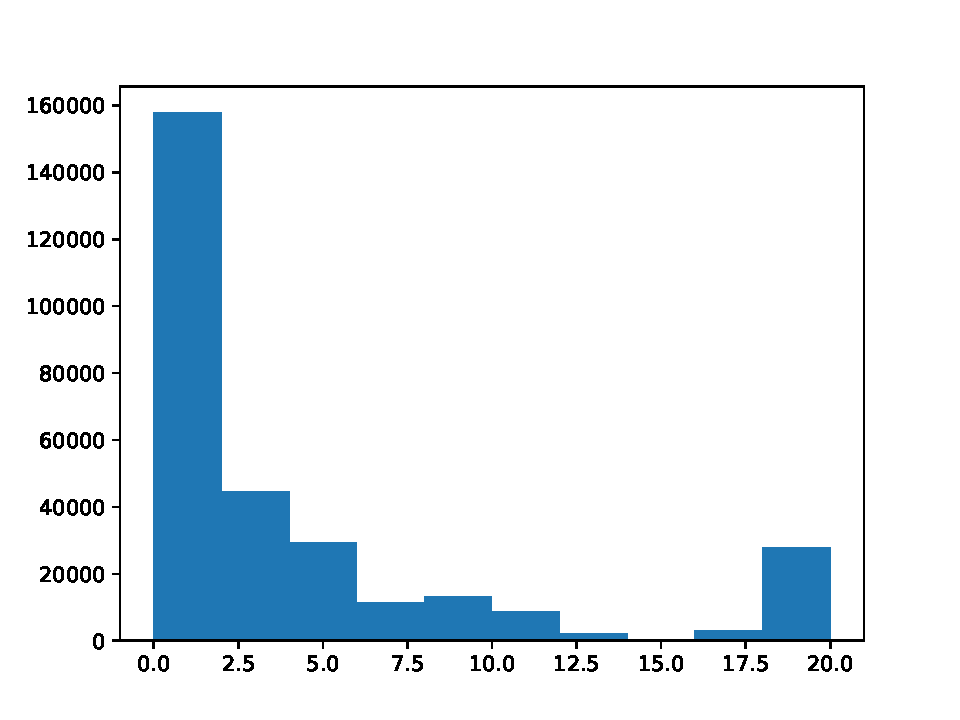
\includegraphics[width=1.11\linewidth]{MBSS/plot/Distribution/2022_02_cores.pdf} 
    \caption{Cores - February 2022} 
    \vspace{4ex}
  \end{minipage} 
  \begin{minipage}[b]{0.5\linewidth}
    \centering
    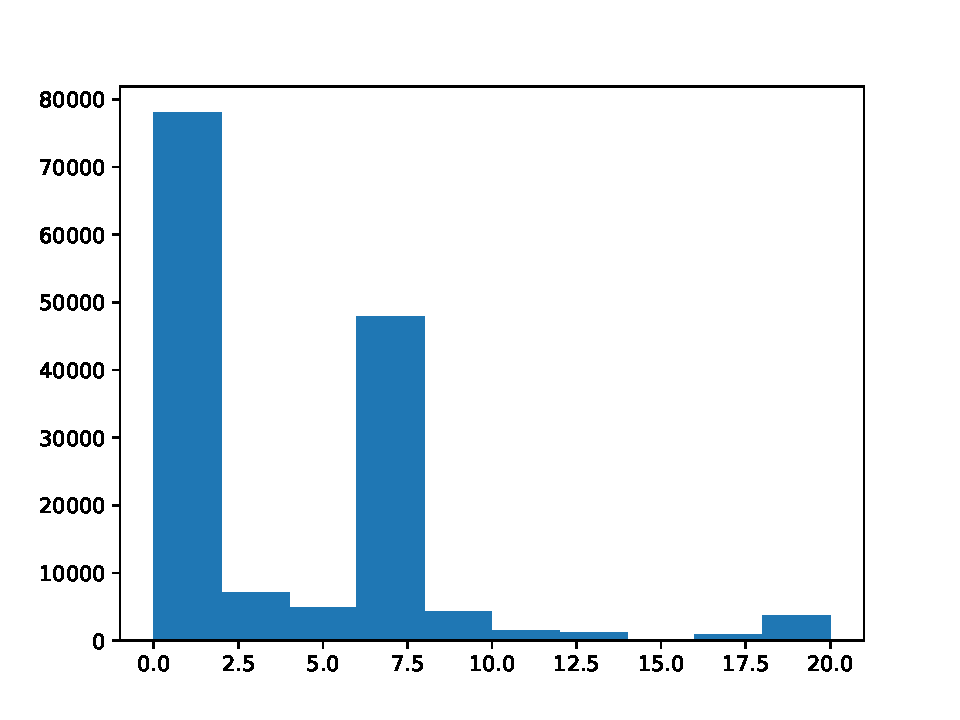
\includegraphics[width=1.11\linewidth]{MBSS/plot/Distribution/2022_03_cores.pdf} 
    \caption{Cores - Mars 2022} 
    \vspace{4ex}
  \end{minipage}%% *
  \begin{minipage}[b]{0.5\linewidth}
    \centering
    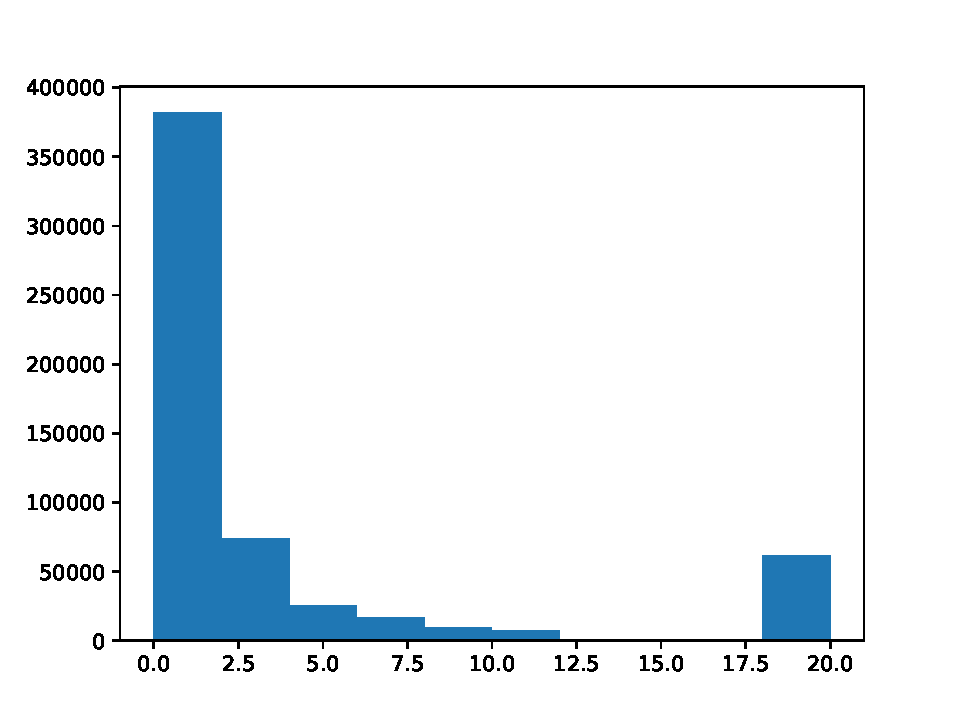
\includegraphics[width=1.11\linewidth]{MBSS/plot/Distribution/2021_12_cores.pdf} 
    \caption{Cores - December 2021} 
    \vspace{4ex}
  \end{minipage}%%
\end{figure}
% Delay
\begin{figure}[H] 
  \begin{minipage}[b]{0.5\linewidth}
    \centering
    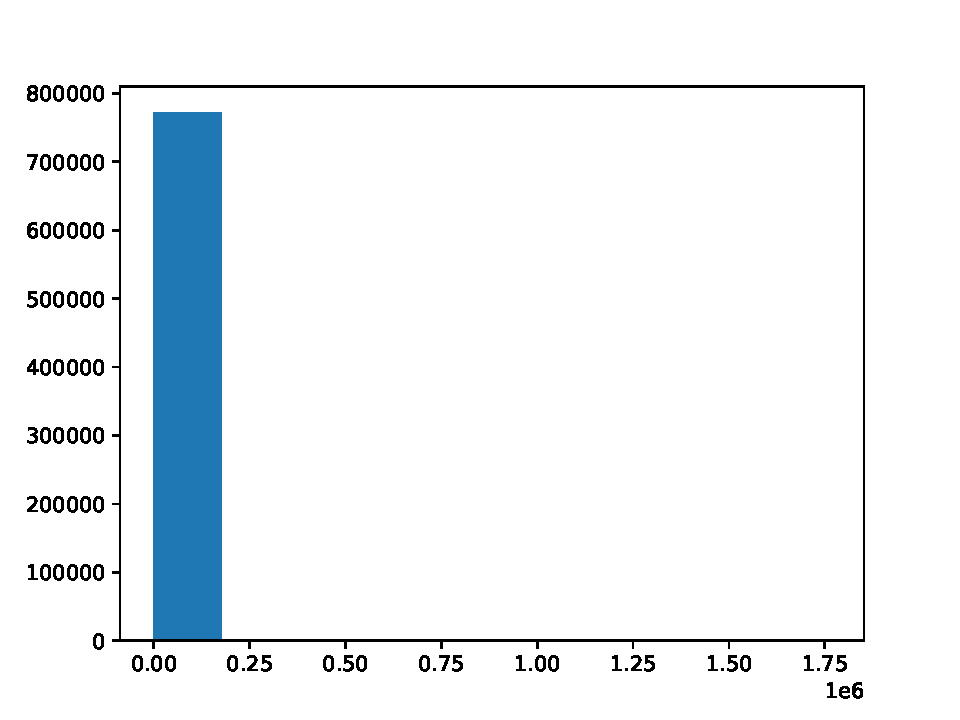
\includegraphics[width=1.11\linewidth]{MBSS/plot/Distribution/2022_01_delay.pdf} 
    \caption{delay - January 2022} 
    \vspace{4ex}
  \end{minipage}%%
  \begin{minipage}[b]{0.5\linewidth}
    \centering
    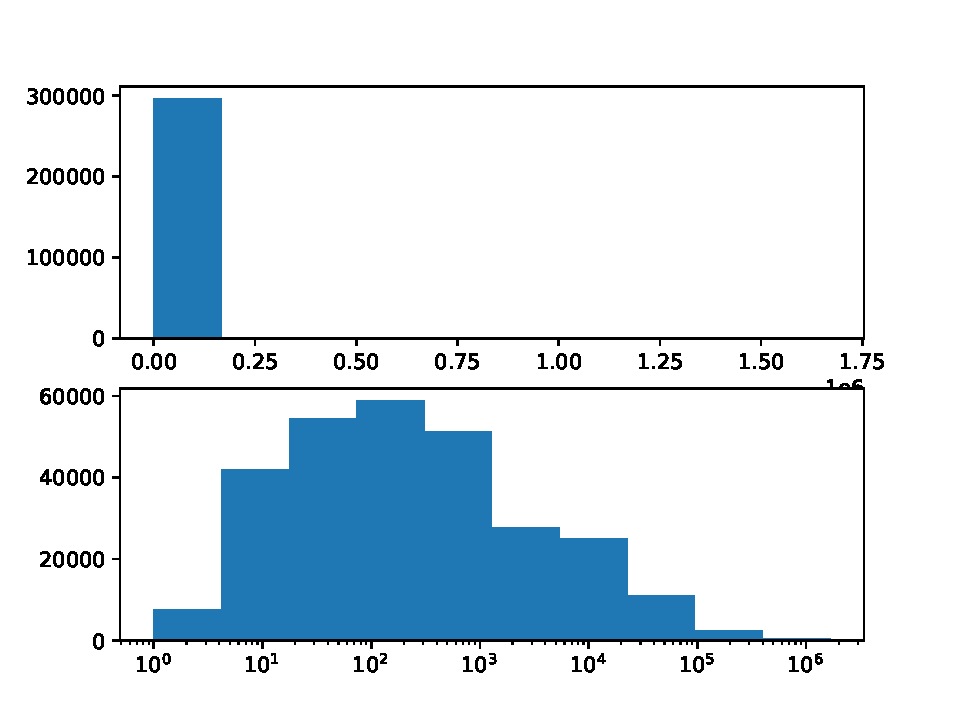
\includegraphics[width=1.11\linewidth]{MBSS/plot/Distribution/2022_02_delay.pdf} 
    \caption{delay - February 2022} 
    \vspace{4ex}
  \end{minipage} 
  \begin{minipage}[b]{0.5\linewidth}
    \centering
    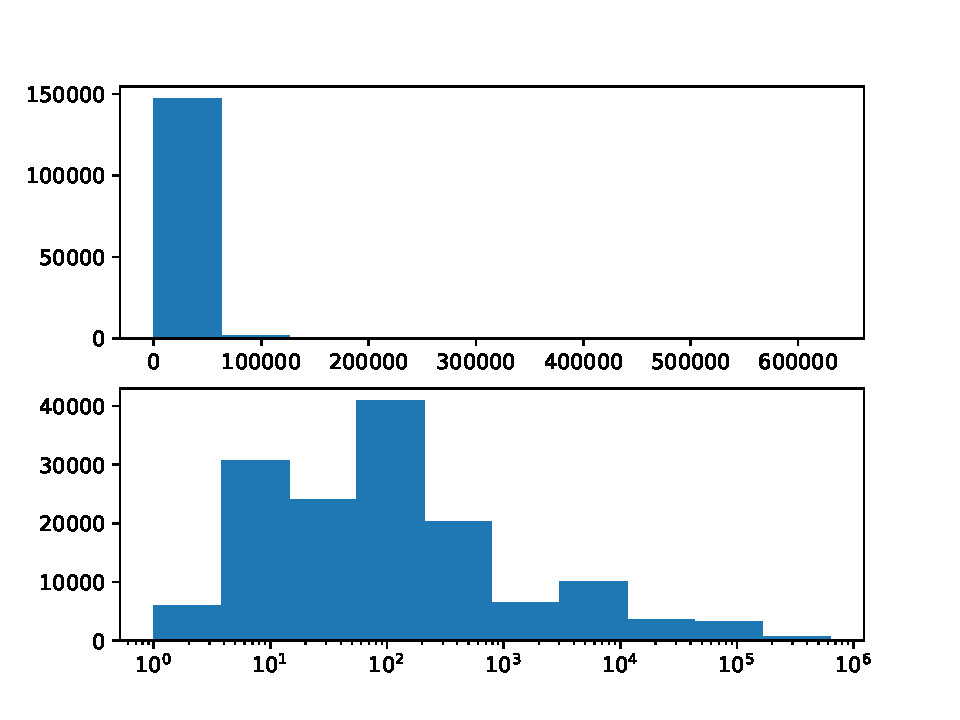
\includegraphics[width=1.11\linewidth]{MBSS/plot/Distribution/2022_03_delay.pdf} 
    \caption{delay - Mars 2022} 
    \vspace{4ex}
  \end{minipage}%% 
    \begin{minipage}[b]{0.5\linewidth}
    \centering
    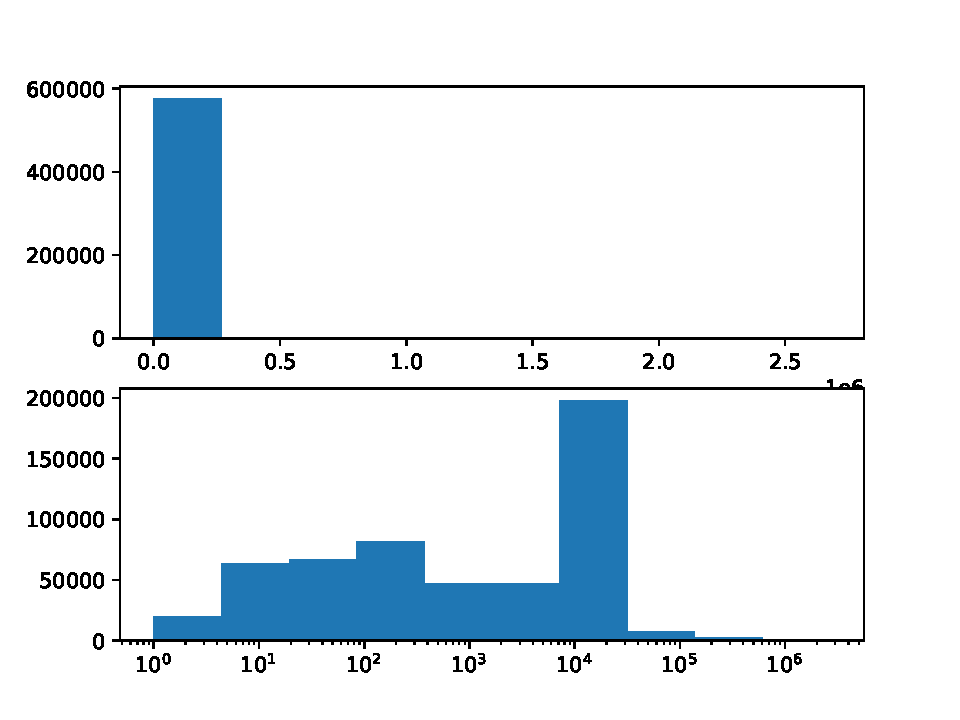
\includegraphics[width=1.11\linewidth]{MBSS/plot/Distribution/2021_12_delay.pdf} 
    \caption{delay - December 2021} 
    \vspace{4ex}
  \end{minipage}%%
\end{figure}
% Walltime
\begin{figure}[H] 
  \begin{minipage}[b]{0.5\linewidth}
    \centering
    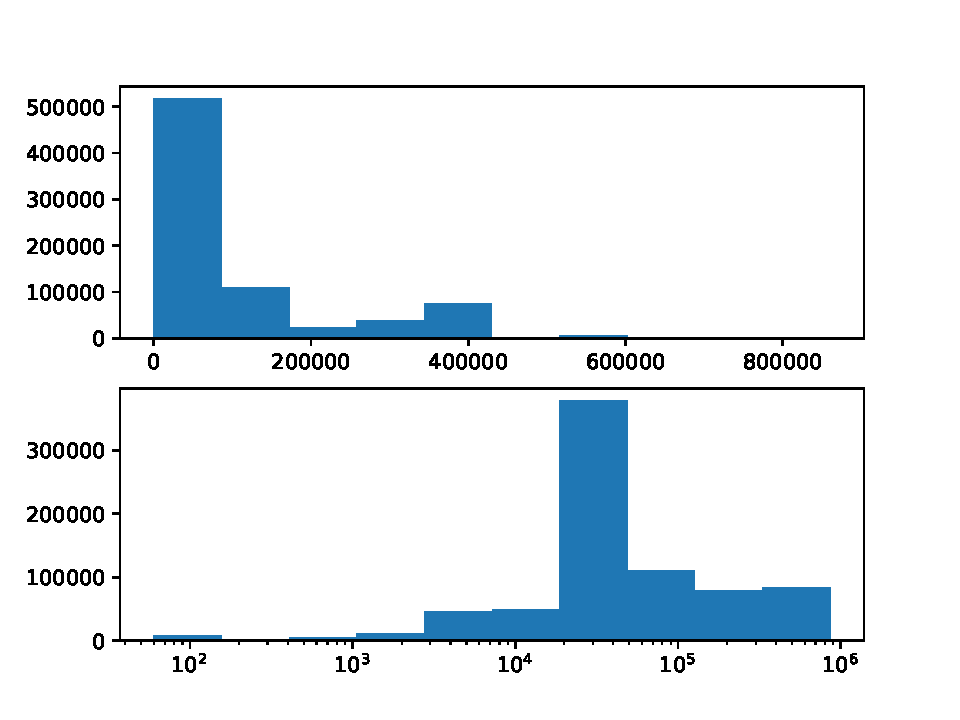
\includegraphics[width=1.11\linewidth]{MBSS/plot/Distribution/2022_01_walltime.pdf} 
    \caption{walltime - January 2022} 
    \vspace{4ex}
  \end{minipage}%%
  \begin{minipage}[b]{0.5\linewidth}
    \centering
    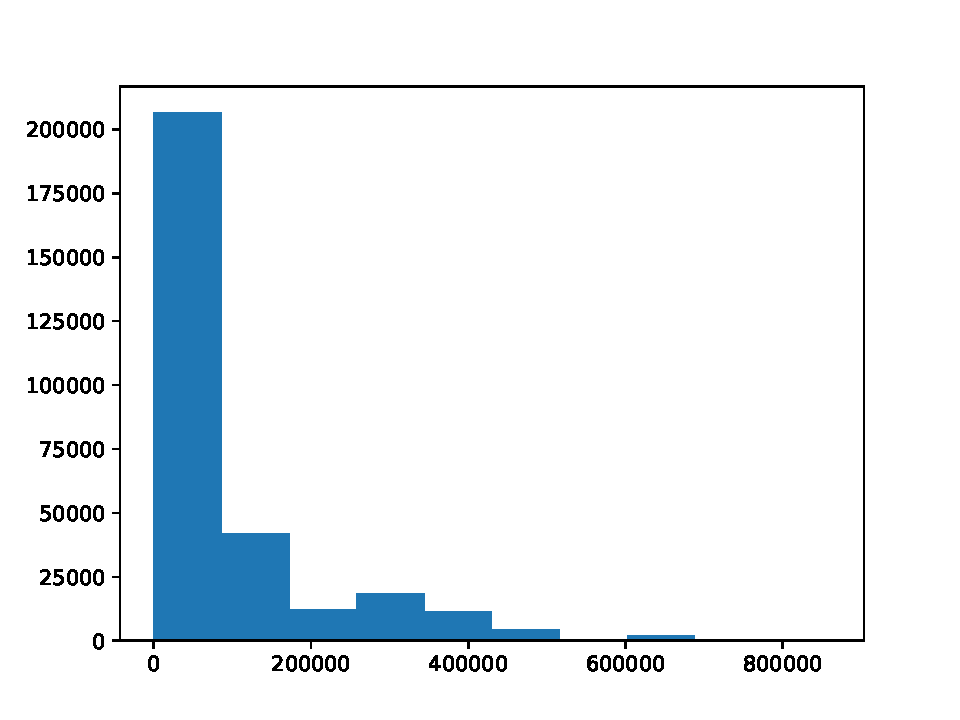
\includegraphics[width=1.11\linewidth]{MBSS/plot/Distribution/2022_02_walltime.pdf} 
    \caption{walltime - February 2022} 
    \vspace{4ex}
  \end{minipage} 
  \begin{minipage}[b]{0.5\linewidth}
    \centering
    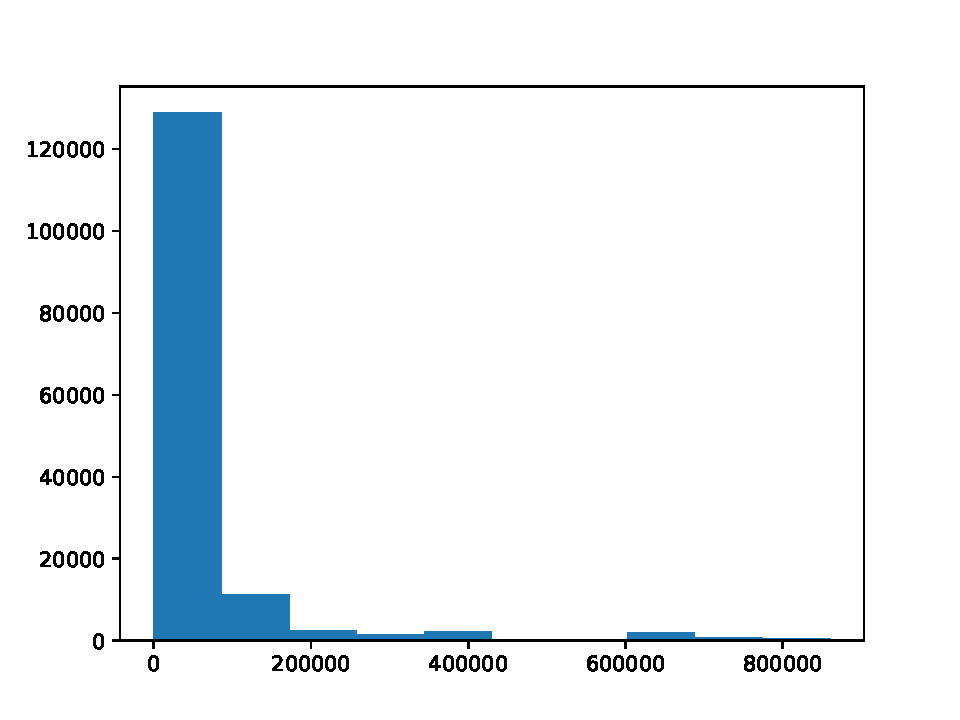
\includegraphics[width=1.11\linewidth]{MBSS/plot/Distribution/2022_03_walltime.pdf} 
    \caption{walltime - Mars 2022} 
    \vspace{4ex}
  \end{minipage}%% 
  \begin{minipage}[b]{0.5\linewidth}
    \centering
    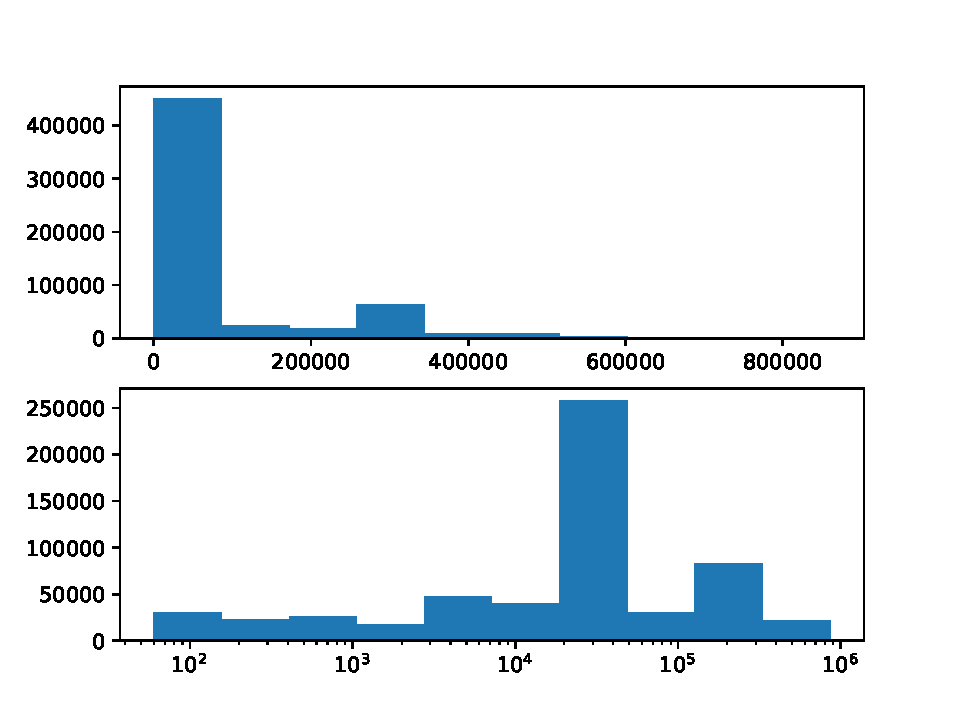
\includegraphics[width=1.11\linewidth]{MBSS/plot/Distribution/2021_12_walltime.pdf} 
    \caption{walltime - Decembre 2021} 
    \vspace{4ex}
  \end{minipage}%%
\end{figure}

\section{Gantt charts}
% Cores
\begin{figure}[H] 
  \begin{minipage}[b]{0.5\linewidth}
    \centering
    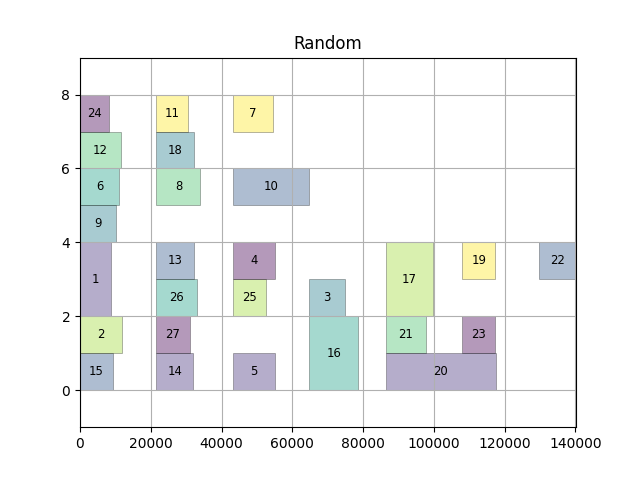
\includegraphics[width=1.11\linewidth]{MBSS/plot/Gantt_charts/Random.png} 
    \caption{Random} 
    \vspace{4ex}
  \end{minipage}%%
\end{figure}

%~ \printbibliography
\end{document}
